\documentclass[12pt, twoside]{article}
\usepackage[letterpaper, margin=1in, headsep=0.5in]{geometry}
\usepackage[english]{babel}
\usepackage[utf8]{inputenc}
\usepackage{amsmath}
\usepackage{amsfonts}
\usepackage{amssymb}
\usepackage{tikz}
\usetikzlibrary{quotes, angles}
\usepackage{graphicx}
\usepackage{enumitem}
\usepackage{multicol}

\newif\ifmeta
\metatrue %print standards and topics tags

\title{Regents Geometry}
\author{Chris Huson}
\date{October 2021}

\usepackage{fancyhdr}
\pagestyle{fancy}
\fancyhf{}
\renewcommand{\headrulewidth}{0pt} % disable the underline of the header
\raggedbottom


\fancyhead[LE]{\thepage}
\fancyhead[RO]{\thepage \\ Name: \hspace{4cm} \,\\}
\fancyhead[LO]{BECA / Dr. Huson / Geometry 03 Parallels and transversals}

\begin{document}

\subsubsection*{3.5 Transversals and angles review}
\begin{enumerate}
\item Do Now: Given two parallel lines and a transversal, as shown, with $m\angle 8 = 123^\circ$.
  \begin{multicols}{2}
    \begin{enumerate}[itemsep=0.5cm]
      \item What angle is corresponding to $\angle 8$?
      \item What angle is alternate exterior to $\angle 8$?
      \item Find $m\angle 2$ \vspace{1cm}
    \end{enumerate}
    \begin{flushright}
      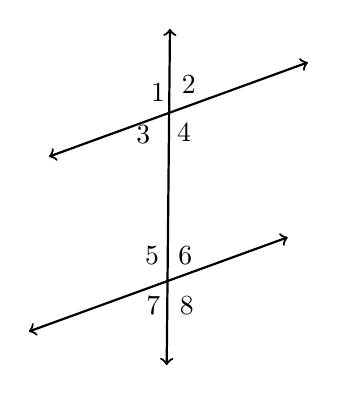
\begin{tikzpicture}[scale=1,rotate=20]
      \draw [<->, thick] (3.5,2)--(7,2);
      \draw [<->, thick] (2.5,0)--(6,0);
      \draw [<->, thick] (4,-1)--(5.5,3);
      \node at (4.5,0.3) [left]{$5$};
      \node at (4.5,0.3) [right]{$6$};
      \node at (4.3,-0.3) [left]{$7$};
      \node at (4.3,-0.3) [right]{$8$};
      \node at (5.2,2) [above left]{$1$};
      \node at (5.2,2.1) [above right]{$2$};
      \node at (5,2) [below left]{$3$};
      \node at (5.1,2) [below right]{$4$};
    \end{tikzpicture}
  \end{flushright}
  \end{multicols}

\item Find $m\angle 1$ given two parallel lines and a transversal, with
  \begin{multicols}{2}
  $\displaystyle m\angle 2 = \frac{2}{7}(2x+58)$ \hspace{0.75cm}$\displaystyle m\angle 7 = \frac{1}{7}(5x+5)$
\begin{flushright}
  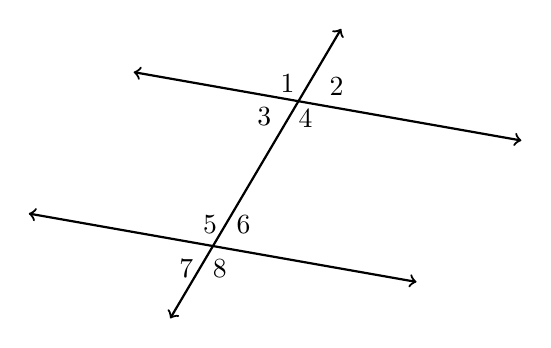
\begin{tikzpicture}[scale=1,rotate=-10]
    \draw [<->, thick] (3,2)--(8,2);
    \draw [<->, thick] (2,0)--(7,0);
    \draw [<->, thick] (4,-1)--(5.5,3);
    \node at (4.5,0.3) [left]{$5$};
    \node at (4.5,0.3) [right]{$6$};
    \node at (4.3,-0.3) [left]{$7$};
    \node at (4.3,-0.3) [right]{$8$};
    \node at (5.2,2) [above left]{$1$};
    \node at (5.4,2) [above right]{$2$};
    \node at (4.9,2) [below left]{$3$};
    \node at (5,2) [below right]{$4$};
  \end{tikzpicture}
\end{flushright} 
\end{multicols} \vspace{2cm}


\item Points that are all located on the same plane are $\rule{4cm}{0.15mm}$.

\item Write down the name of two line segments shown in the diagram below using proper geometric notation.
  \begin{center}
  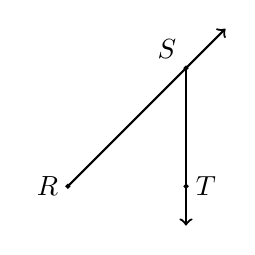
\begin{tikzpicture}[scale=0.5]
    \draw [->, thick] (0,0)--(4,4);
    \draw [->, thick] (3,3)--(3,-1);
    \draw [fill] (0,0) circle [radius=0.05] node[left]{$R$};
    \draw [fill] (3,3) circle [radius=0.05] node[above left]{$S$};
    \draw [fill] (3,0) circle [radius=0.05] node[right]{$T$};
  \end{tikzpicture}
  \end{center}

\item Identify two lines in the given plane.\\[0.25in]
    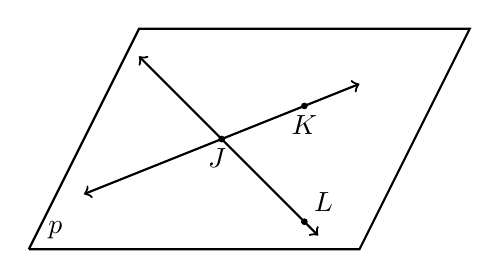
\begin{tikzpicture}[scale=0.7]
      \draw [thick](0,0) node[above right]{$\ p$} --(6,0)--(8,4)--(2,4)--(0,0);
      \draw [<->, thick] (1,1)--(6,3);
      \draw [fill] (3.5,2) circle [radius=0.05] node[below]{$J \ $};
      \draw [fill] (5,2.6) circle [radius=0.05] node[below]{$K$};
      \draw [<->, thick] (2,3.5)--(5.25,.25);
      \draw [fill] (5,0.5) circle [radius=0.05] node[above right]{$L$};
    \end{tikzpicture}

\newpage

\item As shown below, two lines intersect making four angles: $\angle 1$, $\angle 2$, $\angle 3$, and $\angle 4$. Given that $m\angle 1= x+32$ and $m\angle 3=2x-8$, find $m\angle 1$.
  \begin{flushright}
    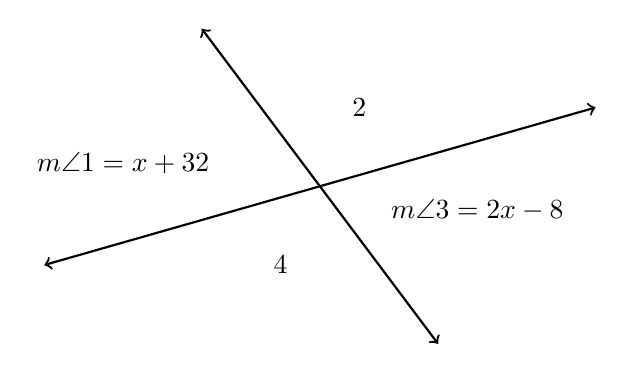
\begin{tikzpicture}[scale=1, rotate=0]
      \draw [<->, thick] (1,-1)--(8,1);
      \draw [<->, thick] (3,2)--(6,-2);
      \node at (2,.3){$m\angle 1= x+32$};
      \node at (6.5,-.3){$m\angle 3=2x-8$};
      \node at (5,1){2};
      \node at (4,-1){4};
    \end{tikzpicture}
    \end{flushright}

\item An angle bisector is shown below, with $\overrightarrow{PR}$ bisecting $\angle QPS$. Given $m\angle QPR = 6x-12$ and $m\angle QPS = 10x+4$, find $m\angle QPS$.
    \begin{flushright}
    \begin{tikzpicture}[scale=0.6, rotate=30]
      \draw [<->, thick] (230:5)node[left]{$Q$} 
      --(0,0)node[above right]{$P$}
      --(110:6)node[above right]{$S$}--(110:7);
      \draw [->, thick] (0,0)--(170:7)node[below right]{$R$};
      %\draw [fill] (0,0) circle [radius=0.05] node[below]{$A$};
      %\draw [fill] (5,0) circle [radius=0.05] node[below]{$B$};
    \end{tikzpicture}
    \end{flushright}

  \item Spicy: Practice these techniques for quadratics ($x^2$)
  \begin{enumerate}[itemsep=2cm]
    \item Expand $(x+4)(x+3)$
    \item Convert to \emph{standard form} (equal to zero): $x^2+4=4x$
    \item Factor, $x^2+9x+8=0$
  \end{enumerate}


\end{enumerate}
\end{document}